% =========================================================================
% WEEK 5 / CHAPTER 10: ELECTRIC FIELDS IN MATTER II
% =========================================================================

\section{Electric Fields in Matter II}

\subsection{The Electric Displacement}

What is $\vb{E}$ generated by a polarized material?
\begin{itemize}
    \item $\vb{E}$ generated by a polarized material $\to$ due to its bound charges.
    \item If ``free charges'' are also present:
    \[
    \text{Total }\vb{E}\text{ is the sum of }\vb{E}_{\text{bound}} + \vb{E}_{\text{free}}.
    \]
\end{itemize}

So in other words:
\begin{equation}
    \div \vb{E} = \frac{\rho}{\varepsilon_0},
\end{equation}
which is Gauss's law in differential form (Maxwell equation \#1). In the case of a polarized dielectric $\rho = \rho_b + \rho_f$, so Eq.~(10.1) becomes:
\begin{equation*}
    \div \vb{E} = \frac{\rho_b + \rho_f}{\varepsilon_0} \implies \div \vb{E} = \frac{1}{\varepsilon_0}\left(-\div \vb{P} + \rho_{\text{free}}\right),
\end{equation*}
from our definition of $\rho_{\text{bound}}$. We can do some algebra to rewrite the equation as:
\begin{equation*}
    \div \underbrace{(\varepsilon_0 \vb{E} + \vb{P})}_{\vb{D}\text{ electric displacement}} = \rho_{\text{free}}
\end{equation*}
\begin{equation}
    \div \vb{D} = \rho_{\text{free}} \quad \text{where} \quad \vb{D} \equiv \varepsilon_0 \vb{E} + \vb{P}
\end{equation}

Then we have that \textbf{Gauss's law for dielectrics} can be written as:
\begin{align*}
    \div \vb{D} &= \rho_{\text{free}} && \text{differential form,} \\
    \intertext{or}
    \oint \vb{D} \cdot \dd{\vb{a}} &= Q_{f,\text{enc}} && \text{integral form.}
\end{align*}

From these expressions it would seem that $\vb{D}$ is the same as $\vb{E}$, but there are significant differences. For example, we know that the curl of $\vb{E}$ is zero (no circulation), but for $\vb{D}$:
\begin{equation}
    \curl \vb{D} = \curl (\varepsilon_0 \vb{E} + \vb{P}) = \varepsilon_0 \underbrace{\curl \vb{E}}_{0} + \curl \vb{P} = \curl \vb{P}.
\end{equation}

Remember that the condition $\curl \vb{E} = \vb{0} \iff \oint \vb{E} \cdot \dd{\vb*{\ell}} = 0$, so we needed this to define the electric potential. The fact that $\vb{D}$ does not satisfy this means that there is \textbf{NO potential function} that generates $\vb{D}$.

Also, the displacement vector $\vb{D}$ is not uniquely determined by $\rho_{\text{free}}$, it requires additional information, for example $\vb{P}$.

\begin{example}[Frozen-in Polarization in a Spherical Shell]
Let's look at the problem we solved last week and see if we can get a quicker answer considering Gauss's law for $\vb{D}$.

A thick spherical shell is made of some material with frozen-in polarization
\[
\vb{P}(\gr) = \frac{k}{r}\,\vu{r},
\]
where $k$ is a constant and $r$ is the distance from the center.

Find the electric field in all regions using $\oint \vb{D} \cdot \dd{\vb{a}} = Q_{f,\text{enc}}$ and then get $\vb{E}$ from the definition of $\vb{D}$.

We have that $\oint \vb{D} \cdot \dd{\vb{a}} = Q_{\text{free}}$; there is no $Q_{\text{free}} \implies \vb{D} = \vb{0}$ everywhere.

Now to find $\vb{E}$:
\[
\vb{D} = \varepsilon_0 \vb{E} + \vb{P} \xrightarrow{\vb{D}=\vb{0}} \varepsilon_0 \vb{E} = -\vb{P} \implies \vb{E} = -\frac{k}{\varepsilon_0 r}\,\vu{r}
\]
for inside the sphere, which is what we had found last time!
\end{example}

\begin{example}[Cavity in a Dielectric]
Suppose the field inside a large piece of dielectric is $\vb{E}_0$, so that the electric displacement is $\vb{D}_0 = \varepsilon_0 \vb{E}_0 + \vb{P}$.

Let's suppose we hollow out the following cavity from the material:
\begin{center}
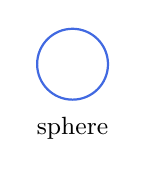
\begin{tikzpicture}
    \draw[thick, RoyalBlue] (0,0) circle (0.45cm);
    \node[below] at (0,-0.55) {\small sphere};
\end{tikzpicture}
\end{center}

Find $\vb{E}$ inside the cavity in terms of $\vb{D}_0$ and $\vb{P}$. Assume the polarization is ``frozen'' (i.e. it doesn't change when the cavity is excavated).

Let's start with the sphere.
Making a spherical cavity is equivalent to superimposing a material with polarization $-\vb{P}$.

Let's calculate the electric field for a sphere with polarization $-\vb{P}$ uniform.

\vspace{0.5em}
\noindent
\begin{minipage}{0.38\textwidth}
\centering
\begin{tikzpicture}[scale=0.85]
    \draw[RoyalBlue, thick] (0, 0.45) circle (1.1);
    \node[RoyalBlue] at (-0.8, 1.1) {\scriptsize $+$};
    \node[RoyalBlue] at (-0.3, 1.3) {\scriptsize $+$};
    \node[RoyalBlue] at (0.3, 1.3) {\scriptsize $+$};
    \node[RoyalBlue] at (0.8, 1.1) {\scriptsize $+$};
    
    \draw[RoyalBlue, thick] (0, -0.45) circle (1.1);
    \node[RoyalBlue] at (-0.8, -1.1) {\scriptsize $-$};
    \node[RoyalBlue] at (-0.3, -1.3) {\scriptsize $-$};
    \node[RoyalBlue] at (0.3, -1.3) {\scriptsize $-$};
    \node[RoyalBlue] at (0.8, -1.1) {\scriptsize $-$};
    
    \draw[-{Latex[length=2mm]}, RoyalBlue, thick] (0, -0.45) -- (0, 0.45) node[midway, left] {$d$};
    \fill[RoyalBlue] (0,-0.45) circle (1.5pt) node[right] {\scriptsize $-$};
    \fill[RoyalBlue] (0,0.45) circle (1.5pt) node[right] {\scriptsize $+$};
\end{tikzpicture}
\par\smallskip\small\textit{Figure 10.1: Two spheres of opposite charge, shifted slightly.}
\end{minipage}
\hfill
\begin{minipage}{0.58\textwidth}
This problem is equivalent to: we have 2 spheres of charge, a positive and a negatively charged one. If we shift them slightly, we need to calculate $\vb{E}$ in the region where the spheres overlap.

How do we do this? Superposition. Let's first calculate it for one sphere.
\end{minipage}

\vspace{0.8em}
\noindent We did this back in lecture 3 or 4:

\noindent
\begin{minipage}{0.38\textwidth}
\centering
\begin{tikzpicture}[scale=0.85]
    \draw[RoyalBlue, thick] (0,0) circle (1.2);
    \draw[dashed, RoyalBlue, thick] (0,0) circle (0.7);
    \draw[-{Latex[length=1.5mm]}, RoyalBlue] (0,0) -- (40:0.7) node[midway, above left=-2pt] {\scriptsize $r$};
    \draw[-{Latex[length=1.5mm]}, RoyalBlue] (0,0) -- (-40:1.2) node[midway, below left=-2pt] {\scriptsize $R$};
    \node[below, align=center] at (0, -1.35) {\scriptsize gaussian\\[-2pt]\scriptsize surface};
\end{tikzpicture}
\par\smallskip\small\textit{Figure 10.2: Gaussian surface inside a sphere.}
\end{minipage}
\hfill
\begin{minipage}{0.58\textwidth}
\begin{align*}
    \oint \vb{E} \cdot \dd{\vb{a}} &= E \left(4\pi r^2\right) = \frac{1}{\varepsilon_0} Q_{\text{enc}} = \frac{1}{\varepsilon_0}\left(\frac{4}{3}\pi r^3 \rho\right) \\
    &\implies \vb{E}_+ = \frac{1}{3\varepsilon_0}\rho\, r_+\, \vu{r}
\end{align*}
for the sphere with $+$ charge, and it should be the same for a sphere of negative charge:
\[
\vb{E}_- = -\frac{\rho}{3\varepsilon_0}\, r_-\, \vu{r}.
\]
\end{minipage}

\vspace{0.8em}
\noindent Now if we overlap the spheres:

\noindent
\begin{minipage}{0.38\textwidth}
\centering
\begin{tikzpicture}[scale=0.85]
    \draw[RoyalBlue, thick] (0, 0.5) circle (1.1);
    \draw[RoyalBlue, thick] (0, -0.5) circle (1.1);
    \coordinate (O1) at (0, 0.5);
    \coordinate (O2) at (0, -0.5);
    \coordinate (P) at (0.2, 0.1);
    
    \draw[-{Latex[length=1.5mm]}, RoyalBlue, thick] (O2) -- (O1) node[midway, right] {\scriptsize $\vb{d}$};
    \draw[-{Latex[length=1.5mm]}, RoyalBlue] (O1) -- (P) node[midway, above left=-2pt] {\scriptsize $\vb{r}_+$};
    \draw[-{Latex[length=1.5mm]}, RoyalBlue] (O2) -- (P) node[midway, below left=-2pt] {\scriptsize $\vb{r}_-$};
\end{tikzpicture}
\par\smallskip\small\textit{Figure 10.3: Overlapping region of two spheres.}
\end{minipage}
\hfill
\begin{minipage}{0.58\textwidth}
For 2 spheres:
\begin{equation}
    \vb{E}_{\text{tot}} = \vb{E}_- + \vb{E}_+ = \frac{\rho}{3\varepsilon_0}(\vb{r}_+ - \vb{r}_-) = -\frac{\rho}{3\varepsilon_0}\vb{d},
\end{equation}
and remembering
\[
\rho = \frac{q}{V} = \frac{q}{\frac{4}{3}\pi R^3} \implies \vb{E}_{\text{tot}} = -\frac{1}{4\pi\varepsilon_0}\frac{q\vb{d}}{R^3},
\]
with $q$ the charge of the $+$ sphere, $\vb{d}$ the vector distance between sphere centers, and $R$ the radius of the sphere.
\end{minipage}

\vspace{0.8em}
So now let's get back to our overlapping spheres. All that we have left is to express Eq.~(10.2) in terms of the polarization of the sphere:
\[
\vb{P} = \frac{\vb{p}}{\text{volume}} \implies \left(\frac{4}{3}\pi R^3\right)\vb{P} = \vb{p} = q\vb{d},
\]
so substituting this in Eq.~(10.2) we have:
\begin{align*}
    \vb{E} &= -\frac{1}{3\varepsilon_0}\vb{P} \quad \text{field for a sphere with polarization }\vb{P}, \\
    \vb{E} &= \frac{\vb{P}}{3\varepsilon_0} \quad \text{if the polarization is negative.}
\end{align*}

Now we can answer the original question. $\vb{E}$ inside will be $\vb{E}_0$ plus $\vb{E}$ due to the sphere:
\[
\implies \vb{E} = \vb{E}_0 + \frac{1}{3\varepsilon_0}\vb{P},
\]
and at the center $\vb{P} = \vb{0}$, so
\[
\vb{D} = \varepsilon_0 \vb{E} = \varepsilon_0 \vb{E}_0 + \frac{\varepsilon_0}{3\varepsilon_0}\vb{P} = \vb{D}_0 - \frac{2}{3}\vb{P}.
\]
\end{example}

\subsection{Linear Dielectrics}

A material is called a \textbf{linear dielectric} if the polarization is linearly proportional to $\vb{E}$:
\begin{equation}
    \vb{P} = \varepsilon_0 \chi_e \vb{E}
\end{equation}
where $\chi_e$ is the \textbf{electric susceptibility}, dimensionless (that's why it's multiplied by $\varepsilon_0$).

So for a linear dielectric:
\begin{align*}
    \vb{D} = \varepsilon_0 \vb{E} + \vb{P} &= \varepsilon_0 \vb{E} + \varepsilon_0 \chi_e \vb{E} = \varepsilon_0 (1 + \chi_e)\vb{E} \\
    &= \varepsilon_0 \underbrace{\varepsilon_r}_{\substack{\text{dielectric}\\\text{constant}}} \vb{E} = \underbrace{\varepsilon}_{\substack{\text{dielectric}\\\text{permittivity}}} \vb{E}
\end{align*}
\[
\therefore \quad \vb{D} = \varepsilon \vb{E}
\]

If the material is isotropic and homogeneous, there will be a relation between free charge density and bound charge density:
\begin{equation*}
    \rho_f = \div \vb{D} = \div (\varepsilon \vb{E}) = \varepsilon_0 \varepsilon_r \div \vb{E} = \varepsilon_0 \varepsilon_r \div \left(\frac{\vb{P}}{\varepsilon_0 \chi_e}\right) = \frac{\varepsilon_r}{\varepsilon_r - 1}\div \vb{P} = -\frac{\varepsilon_r}{\varepsilon_r - 1}\rho_b,
\end{equation*}
\begin{equation*}
    \sigma_b = \vb{P} \cdot \vu{n} = (\vb{D} - \varepsilon_0 \vb{E}) \cdot \vu{n} = \left(\vb{D} - \frac{\vb{D}}{\varepsilon_r}\right) \cdot \vu{n} = \left(\frac{\varepsilon_r - 1}{\varepsilon_r}\right)\vb{D} \cdot \vu{n} = \left(\frac{\varepsilon_r - 1}{\varepsilon_r}\right)\sigma_f.
\end{equation*}

\subsection{Dielectrics Without Battery}

What happens to an electric field due to the presence of a dielectric?

\begin{center}
\begin{minipage}{0.45\textwidth}
\centering
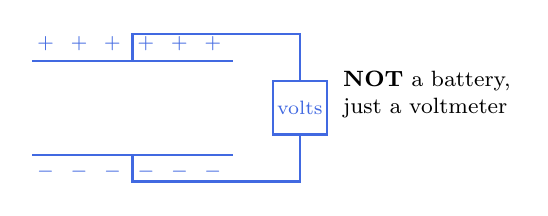
\begin{tikzpicture}[scale=0.85]
    \draw[RoyalBlue, thick] (-2, 0.7) -- (1, 0.7);
    \draw[RoyalBlue, thick] (-2, -0.7) -- (1, -0.7);
    \foreach \x in {-1.8, -1.3, -0.8, -0.3, 0.2, 0.7} {
        \node[RoyalBlue, above] at (\x, 0.7) {\scriptsize $+$};
        \node[RoyalBlue, below] at (\x, -0.7) {\scriptsize $-$};
    }
    \draw[RoyalBlue, thick] (-0.5, 0.7) -- (-0.5, 1.1) -- (2.0, 1.1) -- (2.0, 0.4);
    \draw[RoyalBlue, thick] (-0.5, -0.7) -- (-0.5, -1.1) -- (2.0, -1.1) -- (2.0, -0.4);
    \draw[RoyalBlue, thick] (1.6, -0.4) rectangle (2.4, 0.4);
    \node[RoyalBlue] at (2.0, 0) {\scriptsize volts};
    \node[right, align=left] at (2.5, 0.2) {\footnotesize \textbf{NOT} a battery,\\[-2pt]\footnotesize just a voltmeter};
\end{tikzpicture}
\par\smallskip\small\textit{Figure 10.4: Charged by $V_0$, then battery disconnected.}
\end{minipage}
\hfill
\begin{minipage}{0.45\textwidth}
\centering
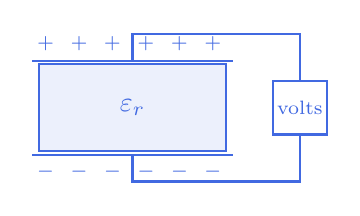
\begin{tikzpicture}[scale=0.85]
    \draw[RoyalBlue, thick] (-2, 0.7) -- (1, 0.7);
    \draw[RoyalBlue, thick] (-2, -0.7) -- (1, -0.7);
    \foreach \x in {-1.8, -1.3, -0.8, -0.3, 0.2, 0.7} {
        \node[RoyalBlue, above] at (\x, 0.7) {\scriptsize $+$};
        \node[RoyalBlue, below] at (\x, -0.7) {\scriptsize $-$};
    }
    \draw[RoyalBlue, thick, fill=RoyalBlue!10] (-1.9, -0.65) rectangle (0.9, 0.65);
    \node[RoyalBlue] at (-0.5, 0) {$\varepsilon_r$};
    \draw[RoyalBlue, thick] (-0.5, 0.7) -- (-0.5, 1.1) -- (2.0, 1.1) -- (2.0, 0.4);
    \draw[RoyalBlue, thick] (-0.5, -0.7) -- (-0.5, -1.1) -- (2.0, -1.1) -- (2.0, -0.4);
    \draw[RoyalBlue, thick] (1.6, -0.4) rectangle (2.4, 0.4);
    \node[RoyalBlue] at (2.0, 0) {\scriptsize volts};
\end{tikzpicture}
\par\smallskip\small\textit{Figure 10.5: Dielectric inserted at constant charge.}
\end{minipage}
\end{center}

\begin{minipage}[t]{0.48\textwidth}
We have a capacitor that we first charge by applying $V_0$.

The capacitor holds a charge $Q_0 = C_0 V_0$.

We disconnect the battery and leave $Q_0 = \text{constant}$.
\end{minipage}
\hfill
\begin{minipage}[t]{0.48\textwidth}
We now put a dielectric inside the capacitor. What happens to $\vb{E}$? Or $V$?

If we measure the potential while keeping the charge constant, we will see that it drops to
\[
V = \frac{V_0}{\varepsilon_r} \quad \text{experimental fact.}
\]
\end{minipage}

\vspace{0.8em}
This means that the capacitance changes in the presence of a dielectric, it is now:
\begin{equation*}
    C = \frac{Q}{V} = \frac{Q_0}{V_0/\varepsilon_r} = \varepsilon_r \frac{Q_0}{V_0} = \varepsilon_r C_0 \quad \therefore \quad \boxed{C = \varepsilon_r C_0}
\end{equation*}

The capacitance is now increased by a factor $\varepsilon_r$.

How do I know it is increasing and not decreasing? For it to decrease $\varepsilon_r < 1$, but by definition $\varepsilon_r = 1 + \chi_e$, so $\varepsilon_r > 1$ since $\chi_e > 0$.

We saw what happens to the capacitance, what happens to the electric field?
\begin{equation*}
    E = \frac{V}{d} = \frac{V_0/\varepsilon_r}{d} = \frac{1}{\varepsilon_r}\left(\frac{V_0}{d}\right) = \frac{E_0}{\varepsilon_r} \quad \therefore \quad \boxed{E = \frac{E_0}{\varepsilon_r}}
\end{equation*}
for a parallel plate capacitor. The field decreases by a factor $\varepsilon_r$.

\subsection{Dielectrics With Battery}

Let's consider the case now in which the battery used to charge the capacitor remains connected as the dielectric is inserted (i.e. in this case we are holding the potential difference constant).

What happens to the charge? Experimentally Faraday found:
\begin{equation}
    Q = \varepsilon_r Q_0,
\end{equation}
where $Q_0$ is the charge on the plates in the absence of dielectric.

\begin{center}
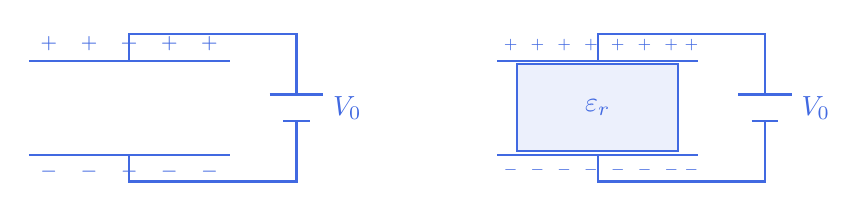
\begin{tikzpicture}[scale=0.85]
    % Left circuit (no dielectric)
    \draw[RoyalBlue, thick] (-5.5, 0.7) -- (-2.5, 0.7);
    \draw[RoyalBlue, thick] (-5.5, -0.7) -- (-2.5, -0.7);
    \foreach \x in {-5.2, -4.6, -4.0, -3.4, -2.8} {
        \node[RoyalBlue, above] at (\x, 0.7) {\scriptsize $+$};
        \node[RoyalBlue, below] at (\x, -0.7) {\scriptsize $-$};
    }
    \draw[RoyalBlue, thick] (-4, 0.7) -- (-4, 1.1) -- (-1.5, 1.1) -- (-1.5, 0.2);
    \draw[RoyalBlue, thick] (-4, -0.7) -- (-4, -1.1) -- (-1.5, -1.1) -- (-1.5, -0.2);
    % Battery symbol
    \draw[RoyalBlue, thick] (-1.9, 0.2) -- (-1.1, 0.2);
    \draw[RoyalBlue, thick] (-1.7, -0.2) -- (-1.3, -0.2);
    \node[right, RoyalBlue] at (-1.1, 0) {$V_0$};
    
    % Right circuit (with dielectric)
    \draw[RoyalBlue, thick] (1.5, 0.7) -- (4.5, 0.7);
    \draw[RoyalBlue, thick] (1.5, -0.7) -- (4.5, -0.7);
    \foreach \x in {1.7, 2.1, 2.5, 2.9, 3.3, 3.7, 4.1, 4.4} {
        \node[RoyalBlue, above] at (\x, 0.7) {\tiny $+$};
        \node[RoyalBlue, below] at (\x, -0.7) {\tiny $-$};
    }
    \draw[RoyalBlue, thick, fill=RoyalBlue!10] (1.8, -0.65) rectangle (4.2, 0.65);
    \node[RoyalBlue] at (3, 0) {$\varepsilon_r$};
    \draw[RoyalBlue, thick] (3, 0.7) -- (3, 1.1) -- (5.5, 1.1) -- (5.5, 0.2);
    \draw[RoyalBlue, thick] (3, -0.7) -- (3, -1.1) -- (5.5, -1.1) -- (5.5, -0.2);
    % Battery symbol
    \draw[RoyalBlue, thick] (5.1, 0.2) -- (5.9, 0.2);
    \draw[RoyalBlue, thick] (5.3, -0.2) -- (5.7, -0.2);
    \node[right, RoyalBlue] at (5.9, 0) {$V_0$};
\end{tikzpicture}
\par\smallskip\small\textit{Figure 10.6: Battery connected ($V_0$ constant, charge increases).}
\end{center}

So then the capacitance becomes:
\begin{equation*}
    C = \frac{Q}{V_0} = \frac{\varepsilon_r Q_0}{V_0} = \varepsilon_r C_0 \quad \therefore \quad \boxed{C = \varepsilon_r C_0}
\end{equation*}
which is the same as we found if the charge is kept constant. But now we are keeping $V$ constant and $Q$ increases.

\subsection{Electric Field of a Parallel Plate Capacitor}

\begin{minipage}{0.48\textwidth}
\centering
\begin{tikzpicture}[scale=0.85]
    \draw[RoyalBlue, thick] (-2, 0.8) -- (2, 0.8) node[left=4.2cm, RoyalBlue] {$+Q$};
    \draw[RoyalBlue, thick] (-2, -0.8) -- (2, -0.8) node[left=4.2cm, RoyalBlue] {$-Q$};
    \foreach \x in {-1.8, -1.4, -1.0, -0.6, -0.2, 0.2, 0.6, 1.0, 1.4, 1.8} {
        \node[RoyalBlue, above] at (\x, 0.8) {\tiny $+$};
        \node[RoyalBlue, below] at (\x, -0.8) {\tiny $-$};
    }
    \draw[dashed, RoyalBlue, thick] (-1, 1.1) rectangle (1, 0.1);
    \node[above, RoyalBlue] at (0, 1.1) {\scriptsize gaussian surface};
    \draw[-{Latex[length=2mm]}, RoyalBlue, thick] (0, 0.1) -- (0, -0.5) node[midway, right] {$\vb{E}_0$};
\end{tikzpicture}
\par\smallskip\small\textit{Figure 10.7: Parallel plate capacitor with no dielectric.}
\end{minipage}
\hfill
\begin{minipage}{0.48\textwidth}
When no dielectric is present we use Gauss's law to calculate the field and get:
\begin{equation*}
    \oint \vb{E} \cdot \dd{\vb{a}} = E_0 A = \frac{Q_{\text{enc}}}{\varepsilon_0} \implies E_0 = \frac{\sigma}{\varepsilon_0},
\end{equation*}
with $\sigma = \dfrac{Q}{A}$.
\end{minipage}

\vspace{1em}

\begin{minipage}{0.48\textwidth}
\centering
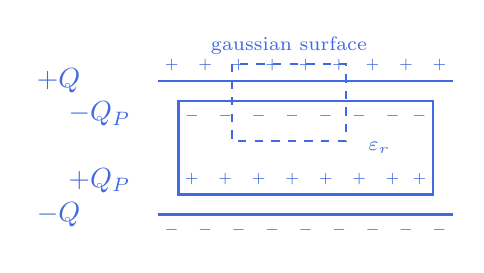
\begin{tikzpicture}[scale=0.85]
    \draw[RoyalBlue, thick] (-2.2, 1.0) -- (2.2, 1.0) node[left=4.6cm, RoyalBlue] {$+Q$};
    \draw[RoyalBlue, thick] (-2.2, -1.0) -- (2.2, -1.0) node[left=4.6cm, RoyalBlue] {$-Q$};
    \foreach \x in {-2.0, -1.5, -1.0, -0.5, 0, 0.5, 1.0, 1.5, 2.0} {
        \node[RoyalBlue, above] at (\x, 1.0) {\tiny $+$};
        \node[RoyalBlue, below] at (\x, -1.0) {\tiny $-$};
    }
    \draw[RoyalBlue, thick] (-1.9, -0.7) rectangle (1.9, 0.7);
    \node[RoyalBlue] at (1.1, 0) {\scriptsize $\varepsilon_r$};
    \foreach \x in {-1.7, -1.2, -0.7, -0.2, 0.3, 0.8, 1.3, 1.7} {
        \node[RoyalBlue, below] at (\x, 0.7) {\tiny $-$};
        \node[RoyalBlue, above] at (\x, -0.7) {\tiny $+$};
    }
    \node[left=2.1cm, RoyalBlue] at (0, 0.5) {$-Q_P$};
    \node[left=2.1cm, RoyalBlue] at (0, -0.5) {$+Q_P$};
    \draw[dashed, RoyalBlue, thick] (-1.1, 1.25) rectangle (0.6, 0.1);
    \node[above, RoyalBlue] at (-0.25, 1.25) {\scriptsize gaussian surface};
\end{tikzpicture}
\par\smallskip\small\textit{Figure 10.8: Bound charges in the dielectric.}
\end{minipage}
\hfill
\begin{minipage}{0.48\textwidth}
What happens now if we throw a dielectric in? Well, we will have some bound charges due to polarization. We can use Gauss's law again:
\begin{align}
    \oint \vb{E} \cdot \dd{\vb{a}} &= EA = \frac{Q_{\text{enc}}}{\varepsilon_0} = \frac{Q - Q_P}{\varepsilon_0} \nonumber \\
    \therefore \quad E &= \frac{Q - Q_P}{\varepsilon_0 A}.
\end{align}
\end{minipage}

\vspace{0.8em}
We just discussed that the effect of the dielectric is to ``weaken'' the original field by a factor $\varepsilon_r$, so setting this equal to expression~(10.3) we get:
\begin{equation}
    E = \frac{E_0}{\varepsilon_r} = \frac{Q}{\varepsilon_r \varepsilon_0 A} = \frac{Q - Q_P}{\varepsilon_0 A},
\end{equation}
so from here we can obtain the amount of bound charge $Q_P$:
\begin{equation}
    \implies Q_P = Q\left(1 - \frac{1}{\varepsilon_r}\right),
\end{equation}
which we can write in terms of surface charge density as
\begin{equation*}
    \sigma_P = \sigma\left(1 - \frac{1}{\varepsilon_r}\right).
\end{equation*}

In the limit $\varepsilon_r \to 1$, $\sigma_P \to 0$, which corresponds to the case of no dielectric.

So now if we substitute the expression for $Q_P$ from Eq.~(10.5) into Eq.~(10.4) we get:
\begin{equation*}
    \oint \vb{E} \cdot \dd{\vb{a}} = \frac{Q}{\varepsilon_r \varepsilon_0} = \frac{Q}{\varepsilon},
\end{equation*}
where $\varepsilon = \varepsilon_r \varepsilon_0$ is the dielectric permittivity, and for a linear dielectric $\vb{D} = \varepsilon \vb{E}$. So the last equation becomes:
\begin{equation*}
    \oint \vb{D} \cdot \dd{\vb{a}} = Q \quad \text{we have arrived again at Gauss's law.}
\end{equation*}

\begin{example}[Capacitance with Dielectrics]
A dielectric of thickness $t$, area $A$ and dielectric constant $\varepsilon_r$ is inserted into the space between the plates of a parallel plate capacitor with spacing $d$, charge $Q$ and area $A$.

What is the capacitance of the system?

\vspace{0.5em}
\noindent
\begin{minipage}{0.48\textwidth}
\centering
\begin{tikzpicture}[scale=0.85]
    \draw[RoyalBlue, thick] (-2, 1.2) -- (2, 1.2);
    \draw[RoyalBlue, thick] (-2, -1.2) -- (2, -1.2);
    \foreach \x in {-1.8, -1.3, -0.8, -0.3, 0.2, 0.7, 1.2, 1.7} {
        \node[RoyalBlue, above] at (\x, 1.2) {\tiny $+$};
        \node[RoyalBlue, below] at (\x, -1.2) {\tiny $-$};
    }
    \draw[RoyalBlue, thick] (-1.5, -0.4) rectangle (1.5, 0.4);
    \node[RoyalBlue] at (0, 0) {\scriptsize $\varepsilon_r$};
    \draw[{Latex[length=1.5mm]}-{Latex[length=1.5mm]}, RoyalBlue] (-2.3, -1.2) -- (-2.3, 1.2) node[midway, left] {$d$};
    \draw[{Latex[length=1.5mm]}-{Latex[length=1.5mm]}, RoyalBlue] (2.3, -0.4) -- (2.3, 0.4) node[midway, right] {$t$};
\end{tikzpicture}
\par\smallskip\small\textit{Figure 10.9: Dielectric of thickness $t$ inside capacitor.}
\end{minipage}
\hfill
\begin{minipage}{0.48\textwidth}
When dealing with capacitors it is helpful to first calculate the potential difference. We have already calculated that in the absence of dielectric the field between the plates is given by
\begin{equation}
    E_0 = \frac{Q}{\varepsilon_0 A},
\end{equation}
and when we add the dielectric:
\begin{equation}
    E_D = \frac{E_0}{\varepsilon_r}.
\end{equation}
\end{minipage}

\vspace{0.8em}
\noindent
\begin{minipage}{0.45\textwidth}
\centering
\begin{tikzpicture}[scale=0.85]
    \draw[RoyalBlue, thick] (-2, 1.5) -- (2, 1.5);
    \draw[RoyalBlue, thick] (-2, -1.5) -- (2, -1.5);
    \foreach \x in {-1.8, -1.3, -0.8, -0.3, 0.2, 0.7, 1.2, 1.7} {
        \node[RoyalBlue, above] at (\x, 1.5) {\tiny $+$};
        \node[RoyalBlue, below] at (\x, -1.5) {\tiny $-$};
    }
    \draw[RoyalBlue, thick] (-1.6, -0.5) rectangle (1.6, 0.5);
    \node[RoyalBlue] at (0.8, 0) {\scriptsize $\varepsilon_r$};
    \draw[-{Latex[length=1.5mm]}, ForestGreen, thick] (0, 1.3) -- (0, 0.7) node[midway, right] {$E_0$};
    \draw[-{Latex[length=1.5mm]}, ForestGreen, thick] (0, 0.3) -- (0, -0.3) node[midway, right] {$E_D$};
    \draw[-{Latex[length=1.5mm]}, ForestGreen, thick] (0, -0.7) -- (0, -1.3) node[midway, right] {$E_0$};
    \draw[{Latex[length=1.5mm]}-{Latex[length=1.5mm]}, RoyalBlue] (-2.3, -1.5) -- (-2.3, 1.5) node[midway, left] {$d$};
    \draw[{Latex[length=1.5mm]}-{Latex[length=1.5mm]}, RoyalBlue] (2.3, -0.5) -- (2.3, 0.5) node[midway, right] {$t$};
\end{tikzpicture}
\par\smallskip\small\textit{Figure 10.10: Fields in the three regions.}
\end{minipage}
\hfill
\begin{minipage}{0.51\textwidth}
The potential can be found by integrating the electric field along a straight line from the top to the bottom of the plates:
\begin{align*}
    V &= -\int_+^- \vb{E} \cdot \dd{\vb*{\ell}} = -V_0 + V_D \\
      &= -E_0(d - t) - E_D t \\
      &= -\frac{Q}{A\varepsilon_0}(d - t) - \frac{Q}{A\varepsilon_0\varepsilon_r}t,
\end{align*}
substituting the expressions (10.6) and (10.7), where $V_D$ is the potential difference between the 2 faces of the dielectric,
\[= -\frac{Q}{A\varepsilon_0}\left[ d - t\left(1 - \frac{1}{\varepsilon_r}\right) \right].\]
\end{minipage}

\vspace{0.8em}
Now that we have the potential difference we can calculate the capacitance:
\begin{equation*}
    \boxed{C = \frac{Q}{V} = \frac{\varepsilon_0 A}{d - t\left(1 - \dfrac{1}{\varepsilon_r}\right)}}
\end{equation*}

It is useful to check the following limits:
\begin{enumerate}
    \item[(i)] As $t \to 0$, i.e. the thickness of the dielectric goes to zero, we get
    \[C = \frac{\varepsilon_0 A}{d} = C_0,\]
    which is what we expect with no dielectric.
    \item[(ii)] As $\varepsilon_r \to 1$ we again have
    \[C \to \frac{\varepsilon_0 A}{d} = C_0,\]
    which is again a situation that corresponds to the dielectric being absent.
    \item[(iii)] In the limit $t \to d$, i.e. the dielectric fills the entire space,
    \[C \to \frac{\varepsilon_r \varepsilon_0 A}{d} = \varepsilon_r C_0.\]
\end{enumerate}

\vspace{0.8em}
\noindent
\begin{minipage}{0.45\textwidth}
\centering
\begin{tikzpicture}[scale=0.85]
    \draw[RoyalBlue, thick] (-2, 1.4) -- (2, 1.4);
    \draw[RoyalBlue, thick] (-2, 0.4) -- (2, 0.4);
    \foreach \x in {-1.8, -1.2, -0.6, 0, 0.6, 1.2, 1.8} {
        \node[RoyalBlue, above] at (\x, 1.4) {\tiny $+$};
        \node[RoyalBlue, below] at (\x, 0.4) {\tiny $-$};
    }
    \draw[-{Latex[length=1.5mm]}, ForestGreen, thick] (0, 1.2) -- (0, 0.6) node[midway, right] {$E_0$};
    \draw[{Latex[length=1.5mm]}-{Latex[length=1.5mm]}, RoyalBlue] (2.2, 0.4) -- (2.2, 1.4) node[midway, right] {$d - t$};
    
    \draw[RoyalBlue, thick] (-2, 0.1) -- (2, 0.1);
    \draw[RoyalBlue, thick] (-2, -1.1) -- (2, -1.1);
    \foreach \x in {-1.8, -1.2, -0.6, 0, 0.6, 1.2, 1.8} {
        \node[RoyalBlue, above] at (\x, 0.1) {\tiny $+$};
        \node[RoyalBlue, below] at (\x, -1.1) {\tiny $-$};
    }
    \draw[RoyalBlue, thick, fill=RoyalBlue!8] (-1.9, -1.0) rectangle (1.9, 0.0);
    \node[RoyalBlue] at (0, -0.5) {\scriptsize $\varepsilon_r$};
    \draw[{Latex[length=1.5mm]}-{Latex[length=1.5mm]}, RoyalBlue] (2.2, -1.1) -- (2.2, 0.1) node[midway, right] {$t$};
\end{tikzpicture}
\par\smallskip\small\textit{Figure 10.11: Two capacitors in series.}
\end{minipage}
\hfill
\begin{minipage}{0.51\textwidth}
Another interesting note: the configuration is equivalent to two capacitors connected in series:
\begin{equation*}
    \frac{1}{C} = \frac{d - t}{\varepsilon_0 A} + \frac{t}{\varepsilon_r \varepsilon_0 A}.
\end{equation*}
This is a good thing to remember when solving problems that involve capacitors and dielectrics.
\end{minipage}
\end{example}

\begin{example}[Capacitor Filled with Two Dielectrics]
Two dielectrics with dielectric constants $\varepsilon_1$ and $\varepsilon_2$ each fill half the space between the plates of a parallel plate capacitor.

\vspace{0.5em}
\noindent
\begin{minipage}{0.45\textwidth}
\centering
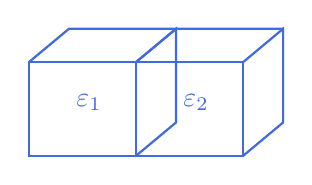
\begin{tikzpicture}[scale=0.85]
    % Simple isometric projection using explicit 2D coords
    % Box 1 (epsilon 1)
    \draw[RoyalBlue, thick] (0,0) -- (1.6,0) -- (1.6,1.4) -- (0,1.4) -- cycle;
    \draw[RoyalBlue, thick] (1.6,0) -- (2.2,0.5) -- (2.2,1.9) -- (1.6,1.4);
    \draw[RoyalBlue, thick] (0,1.4) -- (0.6,1.9) -- (2.2,1.9);
    \node[RoyalBlue] at (0.9, 0.8) {$\varepsilon_1$};
    
    % Box 2 (epsilon 2)
    \draw[RoyalBlue, thick] (1.6,0) -- (3.2,0) -- (3.2,1.4) -- (1.6,1.4);
    \draw[RoyalBlue, thick] (3.2,0) -- (3.8,0.5) -- (3.8,1.9) -- (3.2,1.4);
    \draw[RoyalBlue, thick] (1.6,1.4) -- (2.2,1.9) -- (3.8,1.9);
    \node[RoyalBlue] at (2.5, 0.8) {$\varepsilon_2$};
\end{tikzpicture}
\par\smallskip\small\textit{Figure 10.12: Two dielectrics in parallel.}
\end{minipage}
\hfill
\begin{minipage}{0.51\textwidth}
Each plate has an area $A$ and the plates are separated by a distance $d$.

What is the capacitance of the system?

The potential difference in each half of the capacitor is the same $\implies$ we can think of this system as 2 capacitors connected in parallel.
\end{minipage}

\vspace{0.8em}
For capacitors in parallel, the total capacitance will be:
\begin{equation}
    C = C_1 + C_2,
\end{equation}
so all we need to do is calculate $C_1$ and $C_2$.

From the last discussion we just saw that
\[\frac{1}{C} = \frac{t}{\varepsilon_r \varepsilon_0 A}\]
for a capacitor with a dielectric, where $t$ is the thickness of the dielectric and $A$ the area. So then for this case we have:
\[C_i = \frac{\varepsilon_i \varepsilon_0 (A/2)}{d},\]
because in our case each dielectric only covers half of the area and has a thickness $d$. So substituting these expressions in Eq.~(10.8) we get:
\begin{equation*}
    \boxed{C = \frac{\varepsilon_1 \varepsilon_0 (A/2)}{d} + \frac{\varepsilon_2 \varepsilon_0 (A/2)}{d} = \frac{\varepsilon_0 A}{2d}(\varepsilon_1 + \varepsilon_2)}
\end{equation*}
\end{example}

\subsection{Forces on Dielectrics}

\begin{remark}
\textbf{Demo 429}: Attraction of a dielectric into a capacitor: \url{https://auditoires-physique.epfl.ch/experiment/429}
\end{remark}

A dielectric slab placed partially between the plates of a capacitor will be pulled into the capacitor.

\noindent
\begin{minipage}{0.55\textwidth}
This is a result of the fringing fields around the edges of the capacitor.

The electric field here (at the right edge, denoted by the curved green vectors) cannot be zero, otherwise the line integral along a closed loop at the edge of the capacitor would not be zero.
\end{minipage}
\hfill
\begin{minipage}{0.4\textwidth}
\centering
\begin{tikzpicture}[scale=0.85]
    \draw[RoyalBlue, thick] (-1.8, 1.0) -- (1.0, 1.0);
    \draw[RoyalBlue, thick] (-1.8, -1.0) -- (1.0, -1.0);
    \draw[RoyalBlue, thick, fill=RoyalBlue!10] (-1.5, -0.6) rectangle (0.6, 0.6);
    
    \foreach \x in {-1.2, -0.6, 0, 0.6} {
        \draw[-{Latex[length=1.5mm]}, ForestGreen, thick] (\x, -0.8) -- (\x, 0.8);
    }
    \draw[-{Latex[length=1.5mm]}, ForestGreen, thick] (1.0, -0.8) to[out=60, in=-60] (1.0, 0.8);
    \draw[-{Latex[length=1.5mm]}, ForestGreen, thick] (1.0, -0.9) to[out=40, in=-40] (1.0, 0.9);
\end{tikzpicture}
\par\smallskip\small\textit{Figure 10.13: Fringing fields at capacitor edge.}
\end{minipage}

\vspace{0.8em}
Then we have the following situation:

\noindent
\begin{minipage}{0.45\textwidth}
\centering
\begin{tikzpicture}[scale=0.85]
    % Plates
    \draw[RoyalBlue, thick, fill=RoyalBlue!5] (0, 1.4) -- (2.6, 1.4) -- (3.2, 1.9) -- (0.6, 1.9) -- cycle;
    \draw[RoyalBlue, thick, fill=RoyalBlue!5] (0, 0) -- (2.6, 0) -- (3.2, 0.5) -- (0.6, 0.5) -- cycle;
    
    % Dielectric slab partially inserted
    \draw[thick, ForestGreen, fill=ForestGreen!20] (1.1, 0.2) -- (3.4, 0.2) -- (3.9, 0.65) -- (1.6, 0.65) -- cycle;
    \draw[thick, ForestGreen, fill=ForestGreen!15] (1.1, 1.1) -- (3.4, 1.1) -- (3.9, 1.55) -- (1.6, 1.55) -- cycle;
    \draw[thick, ForestGreen] (1.1, 0.2) -- (1.1, 1.1);
    \draw[thick, ForestGreen] (3.4, 0.2) -- (3.4, 1.1);
    \draw[thick, ForestGreen] (3.9, 0.65) -- (3.9, 1.55);
    \node[ForestGreen] at (2.4, 0.8) {\scriptsize dielectric};
    
    % Dimension markers
    \draw[{Latex[length=1.2mm]}-{Latex[length=1.2mm]}, RoyalBlue] (-0.3, 0) -- (-0.3, 1.4) node[midway, left] {$d$};
    \draw[{Latex[length=1.2mm]}-{Latex[length=1.2mm]}, RoyalBlue] (0, -0.3) -- (2.6, -0.3) node[midway, below] {$w$};
    \draw[{Latex[length=1.2mm]}-{Latex[length=1.2mm]}, RoyalBlue] (0.4, 2.1) -- (-0.2, 1.6) node[midway, above left=-2pt] {$a$};
    \draw[{Latex[length=1.2mm]}-{Latex[length=1.2mm]}, ForestGreen] (1.1, 1.3) -- (2.6, 1.3) node[midway, above] {$s$};
\end{tikzpicture}
\par\smallskip\small\textit{Figure 10.14: Slab with length $s$ inside.}
\end{minipage}
\hfill
\begin{minipage}{0.51\textwidth}
A direct calculation of the $\vb{F}$ requires knowledge of the fringing fields of the capacitor, which are often not well known and difficult to calculate.

An alternative to calculate this $\vb{F}$ is to consider the change in energy of the system when the dielectric is displaced a distance $\dd{s}$.
\end{minipage}

\vspace{0.8em}
The work to be done to move the dielectric an infinitesimal distance $\dd{s}$ is:
\begin{equation*}
    \dd{W} = \vb{F}_{\text{ext}} \cdot \dd{\vb{s}},
\end{equation*}
where $\vb{F}_{\text{ext}}$ is the $\vb{F}$ provided by us to move the slab out of the capacitor. So:
\begin{equation}
    F_{\text{field}} = -F_{\text{ext}} = -\pdv{W}{s}.
\end{equation}

Let's consider the situation shown in the figure where the dielectric is a distance $s$ inside the capacitor. The capacitance of the system is:
\begin{align}
    C &= C_{\text{vac}} + C_{\text{diel}} = \frac{\varepsilon_0(w - s)a}{d} + \frac{\varepsilon_r \varepsilon_0 s a}{d} \nonumber \\
      &= \frac{\varepsilon_0 a}{d}\left(w - s + \varepsilon_r s\right) \nonumber \\
      &= \frac{\varepsilon_0 a}{d}\left[w + (\varepsilon_r - 1)s\right] \nonumber \\
      &= \frac{\varepsilon_0 a}{d}\left[w + \chi_e s\right].
\end{align}

If the total charge on the top plate is $Q$, we know that the energy stored in the capacitor is equal to
\begin{equation*}
    W = \frac{1}{2}\frac{Q^2}{C},
\end{equation*}
so substituting this in Eq.~(10.9) and considering the result of Eq.~(10.10) we get:
\begin{align*}
    F_{\text{field}} &= -\pdv{W}{s} = \frac{1}{2}\frac{Q^2}{C^2}\pdv{C}{s} \quad \text{and} \quad \pdv{C}{s} = \frac{\varepsilon_0 \chi_e a}{d}, \\
    \therefore \quad &\boxed{F_{\text{field}} = \frac{1}{2}\frac{Q^2}{C^2}\frac{\varepsilon_0 \chi_e a}{d} = \frac{1}{2}\frac{\varepsilon_0 \chi_e a}{d}V^2}
\end{align*}

\begin{remark}
Remember, if you ever have questions about the expressions for $\vb{E}$, $\varphi$, etc., look at Fig.~5.2.
\end{remark}